\documentclass{article}
\usepackage{ae,aecompl}
\usepackage{todonotes}
\usepackage{chngcntr}
\usepackage{tikz-cd}
\usepackage{graphicx}
\graphicspath{ {./images/}}
\usepackage[all,cmtip]{xy}
\usepackage{amsmath, amscd}
\usepackage{amsthm}
\usepackage{amssymb}
\usepackage{amsfonts}
\usepackage{bm}
\usepackage{qsymbols}
\usepackage{latexsym}
\usepackage{mathrsfs}
\usepackage{mathtools}
\usepackage{cite}
\usepackage{color}
\usepackage{url}
\usepackage{enumerate}
\usepackage{verbatim}
\usepackage[draft=false, colorlinks=true]{hyperref}
\usepackage{pdfpages}
\usepackage[margin=1.2in]{geometry}
\usepackage{IEEEtrantools}
\usepackage{multirow}
\usepackage{fancyhdr}


\usepackage[nameinlink]{cleveref}


\DeclareMathOperator*{\ac}{accept}
\DeclareMathOperator*{\amax}{argmax}
\DeclareMathOperator*{\amin}{argmin}
\DeclareMathOperator*{\Aut}{Aut}
\newcommand {\al}{{\alpha}}
\newcommand {\abs}[1]{{\left\lvert#1\right\rvert}}
\newcommand {\A}{{\mathcal{A}}}
\newcommand {\AM}{{\mathrm{AM}}}
\newcommand {\AMp}{{\AM_{p}^{X}\!(\Ri_\w)}}
\newcommand {\B}{{\mathcal{B}}}
\DeclareMathOperator*{\Be}{Bern}
\newcommand {\Br}{{\dot{B}}}
\newcommand {\Ba}{{\mathfrak{B}}}
\newcommand {\C}{{\mathbb C}}
\newcommand {\ce}{\mathrm{c}}
\newcommand {\Ce}{\mathrm{C}}
\newcommand {\Cc}{\mathrm{C_{c}}}
\newcommand {\Ccinf}{\mathrm{C_{c}^{\infty}}}
\DeclareMathOperator{\DEV}{DEV}
\DeclareMathOperator{\diag}{diag}
\newcommand {\Di}{{\mathbb D}}
\newcommand {\dom}{\mathrm{dom}}
\newcommand {\ud}{\mathrm{d}}
\newcommand {\ue}{\mathrm{e}}
\newcommand {\eps}{\varepsilon}
\newcommand {\veps}{\varepsilon}
\newcommand {\vrho}{{\varrho}}
\newcommand {\E}{{\mathbb{E}}}
\newcommand {\Ec}{{\mathcal{E}}}
\newcommand {\Ell}{L}
\newcommand {\Ellp}{{L_{p}[0,1]}}
\newcommand {\Ellpprime}{{L_{p'}([0,1])}}
\newcommand {\Ellq}{{L_{q}([0,1])}}
\newcommand {\Ellqprime}{{L_{q'}([0,1])}}
\newcommand {\Ellr}{L^{r}}
\newcommand {\Ellone}{{L_{1}([0,1])}}
\newcommand {\Elltwo}{{L_{2}([0,1])}}
\newcommand {\Ellinfty}{L^{\infty}}
\newcommand {\Ellinftyc}{L_{\mathrm{c}}^{\infty}}
\newcommand {\exb}[1]{\exp\left\{#1\right\}}
\DeclareMathOperator*{\Exp}{Exp}
\DeclareMathOperator*{\Ext}{Ext}
\newcommand {\F}{{\mathcal{F}}}
\newcommand{\Fe}{{\mathbb{F}}}
\newcommand
{\G}{{\mathcal{G}}}
\newcommand {\HF}{\mathcal{H}_{\text{FIO}}^{1}(\Rd)}
\newcommand {\Hr}{H}
\newcommand {\HT}{\mathcal{H}}
\newcommand {\ui}{\mathrm{i}}
\newcommand {\I}{{I}}
\newcommand {\J}{{\mathcal{J}}}
\newcommand {\id}{{\mathrm{id}}}
\newcommand {\iid}{\stackrel{\mathclap{\normalfont\mbox{iid}}}{\sim}}
\newcommand {\im}{{\text{im }}}
\newcommand {\ind}{{\perp\!\!\!\perp}}
\newcommand{\indep}{\stackrel{\text{Indep}}{\sim}}
\DeclareMathOperator*{\Int}{int}
\newcommand {\intx}{{\overline{\int_{X}}}}
\newcommand {\inte}{{\overline{\int_{\E}}}}
\newcommand {\la}{\lambda}
\newcommand {\rb}{\rangle}
\newcommand {\lb}{{\langle}}
\newcommand {\La}{\Lambda}
\newcommand {\calL}{{\mathcal{L}}}
\newcommand {\lp}{{\mathcal{L}}^{p}}
\newcommand {\lpo}{{\overline{\mathcal{L}}^{p}\!}}
\newcommand {\Lpo}{{\overline{\Ell}^{p}\!}}
\newcommand {\M}{{\mathbf{M}}}
\newcommand {\Ma}{{\mathcal{M}}}
\newcommand {\N}{{{\mathbb N}}}
\newcommand {\Na}{{{\mathcal{N}}}}
\newcommand {\norm}[1]{\left\|#1\right\|}
\newcommand {\normm}[1]{{\left\vert\kern-0.25ex\left\vert\kern-0.25ex\left\vert #1 
    \right\vert\kern-0.25ex\right\vert\kern-0.25ex\right\vert}}
\newcommand {\Om}{{{\Omega}}}
\newcommand {\one}{{{\bf 1}}}
\newcommand {\pic}{\text{Pic }}
\newcommand {\ph}{{\varphi}}
\newcommand {\Pa}{{\mathbb{P}}}
\newcommand {\Po}{{\mathcal{P}}}
\newcommand {\Q}{{\mathbb{Q}}}
\newcommand {\R}{{\mathbb R}}
\newcommand {\Rd}{{\mathbb{R}^{d}}}
\DeclareMathOperator{\rej}{reject }
\newcommand {\Rn}{{\mathbb{R}^{n}}}
\newcommand {\cR}{{\mathcal{R}}}
\newcommand {\Rad}{{\mathrm{Rad}}}
\newcommand {\ran}{{\mathrm{ran}}}
\newcommand {\Ri}{{\mathrm{R}}}
\newcommand {\supp}{{\mathrm{supp}}}
\newcommand {\Se}{\mathrm{S}}
\newcommand {\Sp}{S^{*}(\Rn)}
\newcommand {\St}{{\mathrm{St}}}
\newcommand {\Sw}{\mathcal{S}}
\newcommand {\T}{{\mathcal{T}}}
\newcommand {\ta}{{\theta}}
\newcommand {\Ta}{{\Theta}}
\DeclareMathOperator {\V}{Var}
\newcommand {\w}{{\omega}}
\newcommand {\W}{{\mathrm{W}}}
\newcommand {\Wnp}{\text{$\mathrm{W}$\textsuperscript{$n,\!p$}}}
\newcommand {\Wnpeq}{\text{$\mathrm{W}$\textsuperscript{$n\!,\!p$}}}
\newcommand {\Wonep}{\text{$\mathrm{W}$\textsuperscript{$1,\!p$}}}
\newcommand {\Wonepeq}{\text{$\mathrm{W}$\textsuperscript{$1\!,\!p$}}}
\newcommand {\X}{{\mathcal{X}}}
\newcommand {\Z}{{{\mathbb Z}}}
\newcommand {\Za}{{\mathcal{Z}}}
\newcommand {\Zd}{{\Z[\sqrt{d}]}}
\newcommand {\vanish}[1]{\relax}

\newcommand {\wh}{\widehat}
\newcommand {\wt}{\widetilde}
\newcommand {\red}{\color{red}}

% Distributions
\newcommand{\normal}{\mathsf{N}}
\newcommand{\poi}{\mathsf{Poisson}}
\newcommand{\bern}{\mathsf{Bernoulli}}
\newcommand{\bin}{\mathsf{Binomal}}
\newcommand{\multi}{\mathsf{Multinomial}}




% put your command and environment definitions here




% some theorem environments
% remove "[theorem]" if you do not want them to use the same number sequence


  \newtheorem{thrm}{Theorem}
  \newtheorem{lemma}{Lemma}
  \newtheorem{prop}{Proposition}
  \newtheorem{cor}{Corollary}

  \newtheorem{conj}{Conjecture}
  \renewcommand{\theconj}{\Alph{conj}}  % numbered A, B, C etc

  \theoremstyle{definition}
  \newtheorem{defn}{Definition}
  \newtheorem{ex}{Example}
  \newtheorem{exs}{Examples}
  \newtheorem{question}{Question}
  \newtheorem{remark}{Remark}
  \newtheorem{notn}{Notation}
  \newtheorem{exer}{Exercise}




\title{STATS 305 A - Lecture 3}
\author{John Duchi\\ Scribed by Michael Howes}
\date{09/28/21}

\pagestyle{fancy}
\fancyhf{}
\rhead{STATS305A - Lecture 3}
\lhead{09/28/21}

\begin{document}
\maketitle
\tableofcontents

\section{Announcements}
\begin{itemize}
    \item Homowork 1 to be posted tonight. Due in two weeks. An email notice will be sent.
    \item TA's office hours times available on the website.
    \item John's office hours TBD.
    \item First Etude will probably be posted on Friday. Each etude will be checked/attempted by the TAs.
    \item R and python and maybe Julia will be supported for assignments.
\end{itemize}

\section{Recap/Linear Algebra (SVD)}
\subsection{SVD in statistics}
Recall that if $A \in \R^{m \times n}$ and $m \ge n$ ($A$ is tall), then $A$ has a singular value decompsition (SVD) as 
\[A = U\Sigma V^T, \]
where $U \in \R^{m \times n}$ (same size as $A$ and thus also tall), $\Sigma = \diag(s_1,\ldots,s_n) \in \R^{n \times}$ and $s_1 \ge s_2 \ge \ldots \ge s_n \ge 0$, $V \in \R^{n \times n}$ and $U^TU = V^TV = I_n$.

We can give a statistical interpretation of the SVD. Suppose we have the linear model $Y = X\beta+\varepsilon$ where $\varepsilon \sim (0,\sigma^2I_n)$, $X \in \R^{n \times d}$ and $n \ge d$ ($X$ is tall and we have more observations than variables). Then $X = U\Sigma V^T$ with $\Sigma = \diag(s_1,\ldots, s_d)$, $U= [u_1,\ldots, u_d]$ and $v = [v_1,\ldots,v_d]$. Our goal is to recover information about $\beta$ from the data $(X,Y)$.

The components of $\beta$ in the $v_d$ directions are ``hard'' to infer anything about. To make this precise, consider
\[\beta_0 \text{ and }\beta_t = \beta_0-tv_d. \]
Then
\begin{IEEEeqnarray*}{rCl}
    X\beta_0 - X\beta_t &=& -tXv_d\\
    &=&-tU\begin{bmatrix}
        s_1&0&\ldots&0\\
        0&s_2&\ldots&0\\
        \vdots&\vdots&\ddots&\vdots\\
        0&0&\ldots&s_d
    \end{bmatrix}\begin{bmatrix}
        0\\0\\ \vdots \\ 1
    \end{bmatrix}\\
    &=&-ts_du_d,
\end{IEEEeqnarray*}
since $Vv_d=e_d$. Thus we need $t \sim \frac{1}{s_d}$ to induce substantial changes to the observed $Y$. Constrast this with making inferences in the $v_1$ direction. If $\beta_t = \beta_0 - tv_1$, then  $X\beta_0 - X\beta_t = ts_1u_1$. Thus changes in the $v_1$ direction give us relatively big changes in $Y$.

Note that the singular values are always non-negative.
\subsection{A concrete exmaple}
[In answer to a question] Historically linear models were developed for agriculture where $Y_i = \text{yield in kg of field }i$ and
\[X = \begin{bmatrix}
    \horzbar&X_1^T&\horzbar\\\
    &\vdots&\\
    \horzbar&X_n^T&\horzbar
\end{bmatrix}, \]
where $X_i \in \{0,1\}^d$ encodes the treatments given to field $i$ and in particular $X_{i,j} = 1$ if treatment $j$ was used in field $i$.

\subsection{Geometric interpretation of SVD}
[In answer to another question] Suppose $A = U\Sigma V^t$, then $Ax = U\Sigma Vx$, thus we can calculate $Ax$ in three successive steps.
\begin{enumerate}
    \item[(Step 1)] First 
    \[V^Tx = \begin{bmatrix}
        v_1^Tx\\
        \vdots\\
        v_n^Tx
    \end{bmatrix} \]
    are the coordinates of $x$ in the basis $V$.
    \item[(Step 2)] We apply $s_i$ gains to the components of $Vx$
    \[\Sigma V^Tx = \begin{bmatrix}
        s_1v_1^Tx\\
        \vdots\\
        s_nv_n^Tx
    \end{bmatrix}.  \]   
    \item[(Step 3)] We use these values to define a new vector using the basis $U$.
    \[Ax = U\Sigma V^Tx = U\begin{bmatrix}
        s_1v_1^Tx\\
        \vdots\\
        s_nv_n^Tx
    \end{bmatrix} = \sum_{i=1}^n (s_iv_i^Tx)u_i.  \]  
\end{enumerate}
Here is a picture of these steps.

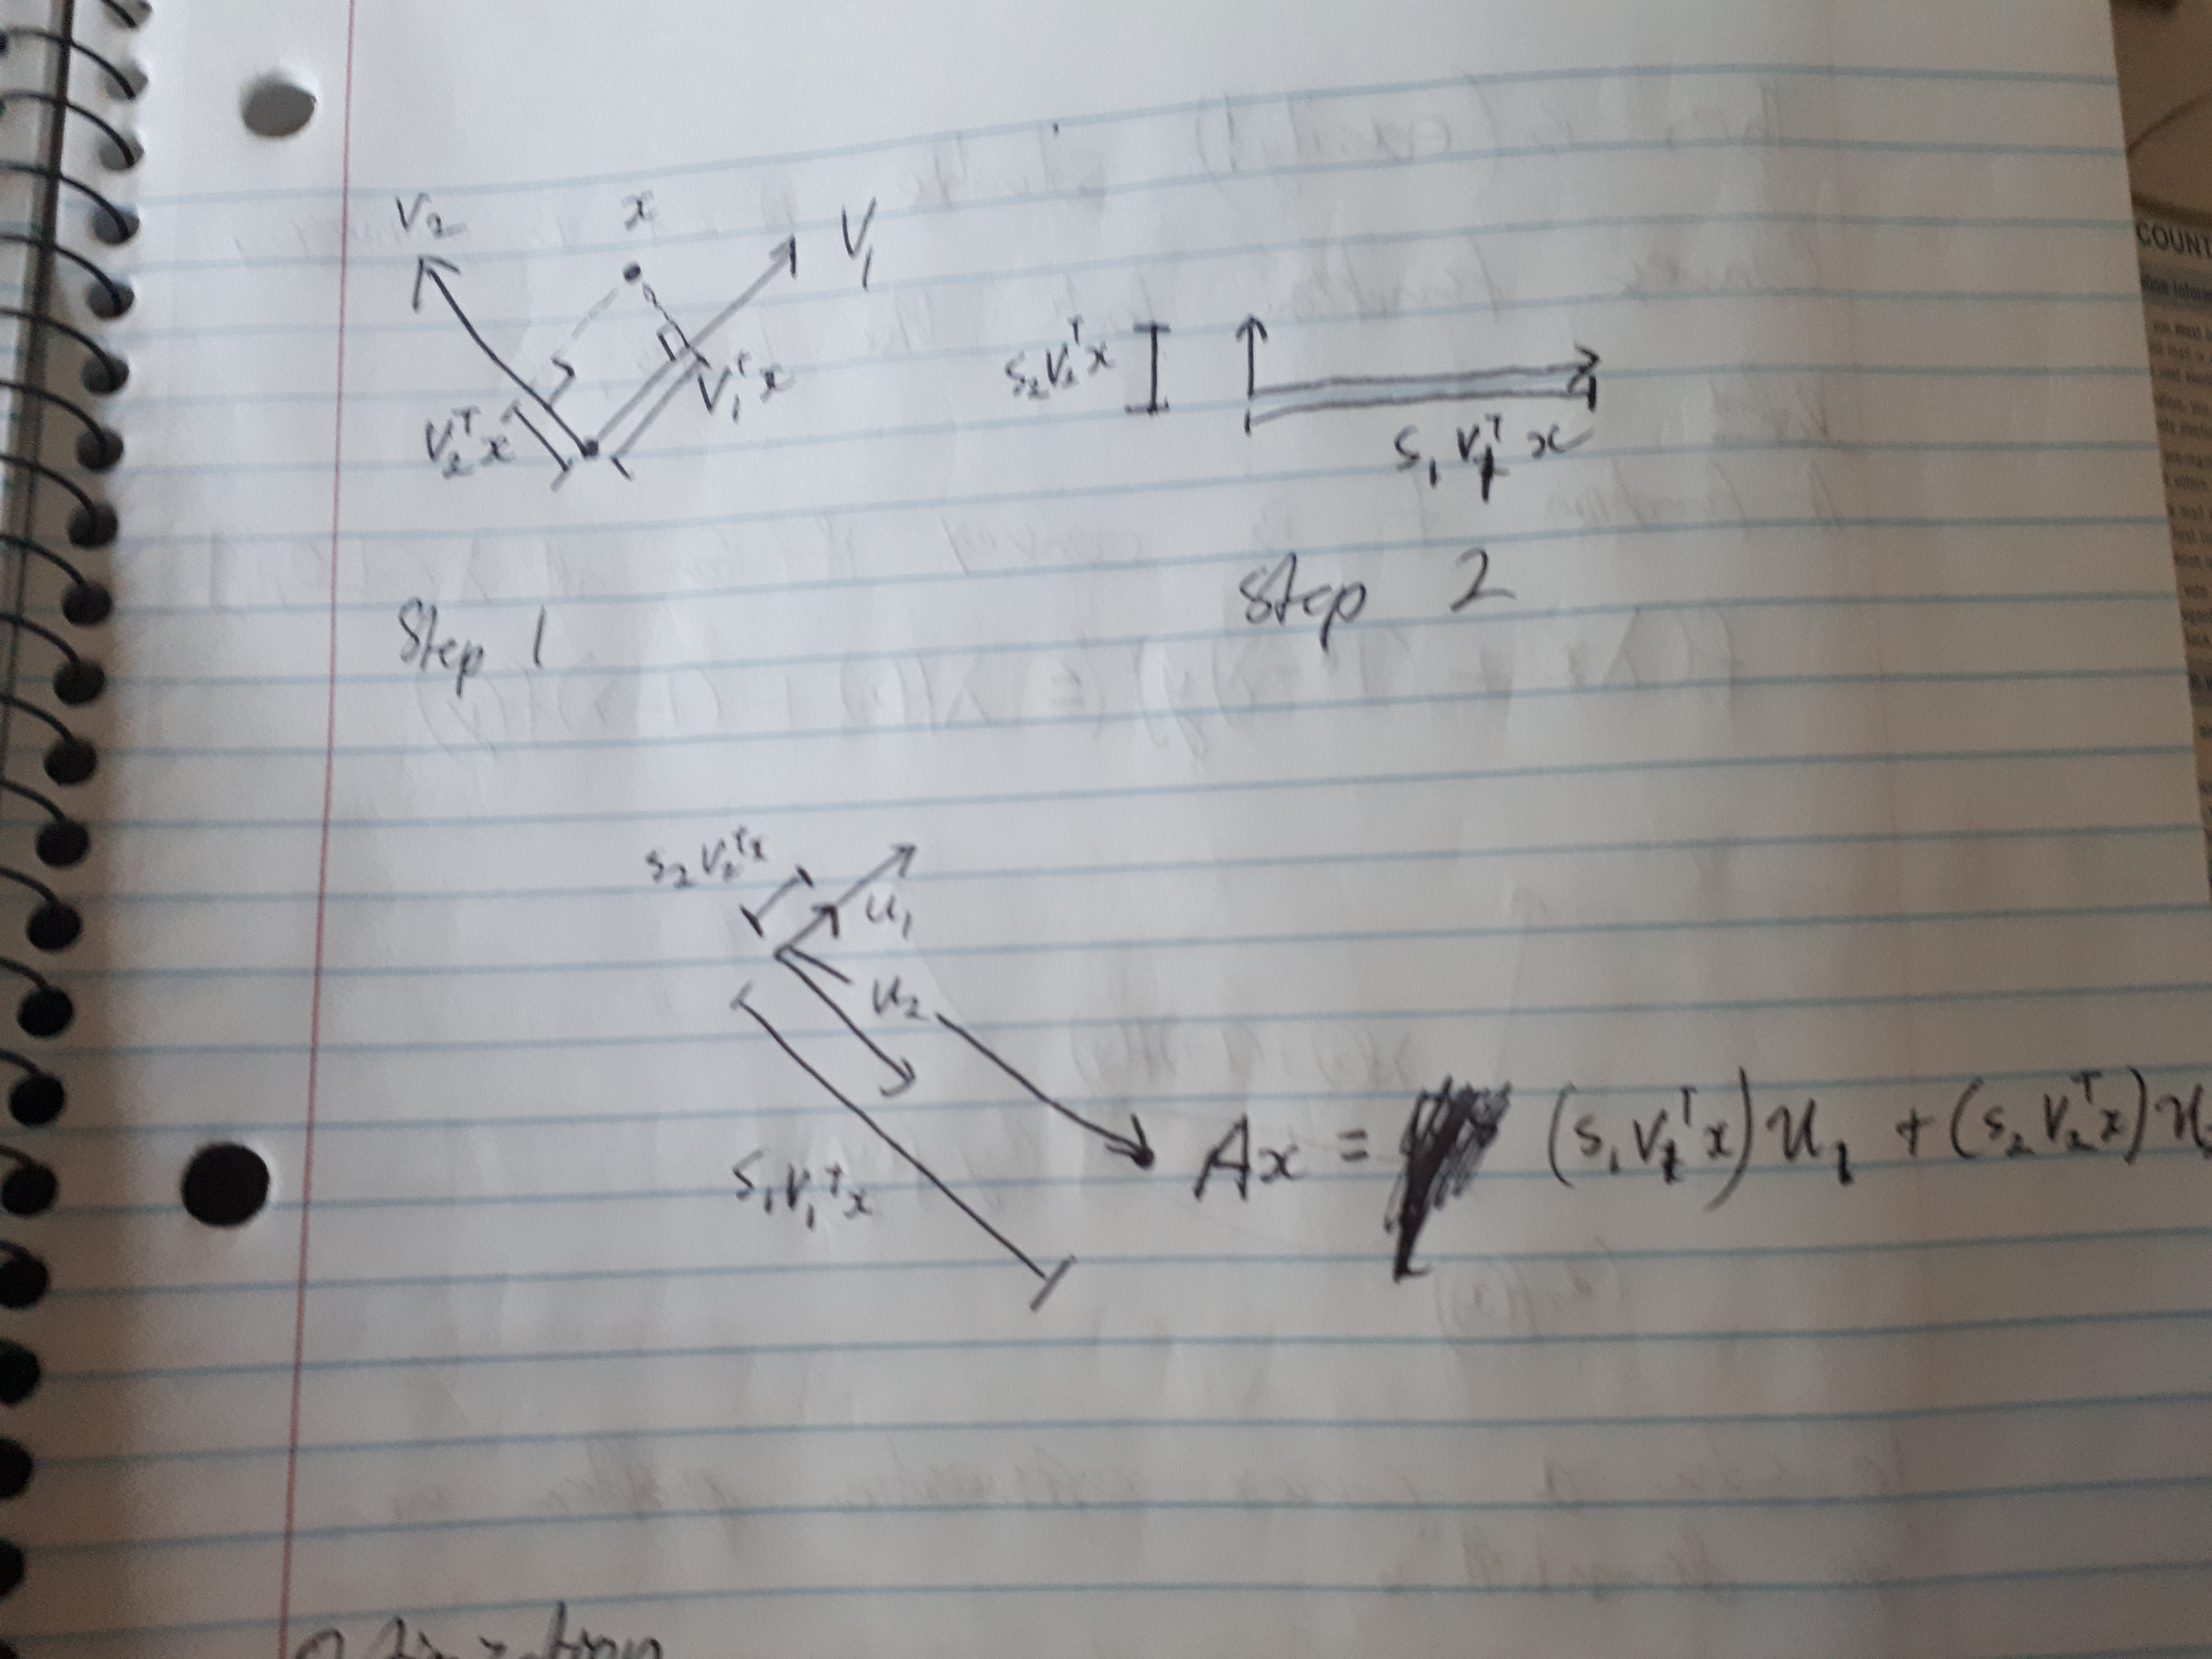
\includegraphics[width = \textwidth]{09_28_P01.jpg}
\section{Optimisation Basics}
\subsection{Convex Optimisation}
Optimisation is about problems of the form minimize $f(x)$ s.t $h(x) = 0$ and $g(x) \le 0$. The function $f$ is our objective, $x$ is out variable, $h$ is an equality constraint and $g$ are inequality constraints. In this class we will mostly consider unconstrained cases.

This is solvable (easily!) is $f$ is \emph{convex}. If $f$ isn't \emph{convex} we are in trouble. Convex functions look like bowls.

\begin{defn}
    A function $f$ is convex if for all $\la \in [0,1]$
    \[f(\la x + (1-\la)y) \le \la f(x)+(1-\la)f(y). \]
    That is if we graph $f$, then the line between $(x,f(x))$ and $(y,f(y))$ lies above the graph of $f$ (bowl shaped). (See picture)
\end{defn}

\begin{center}
    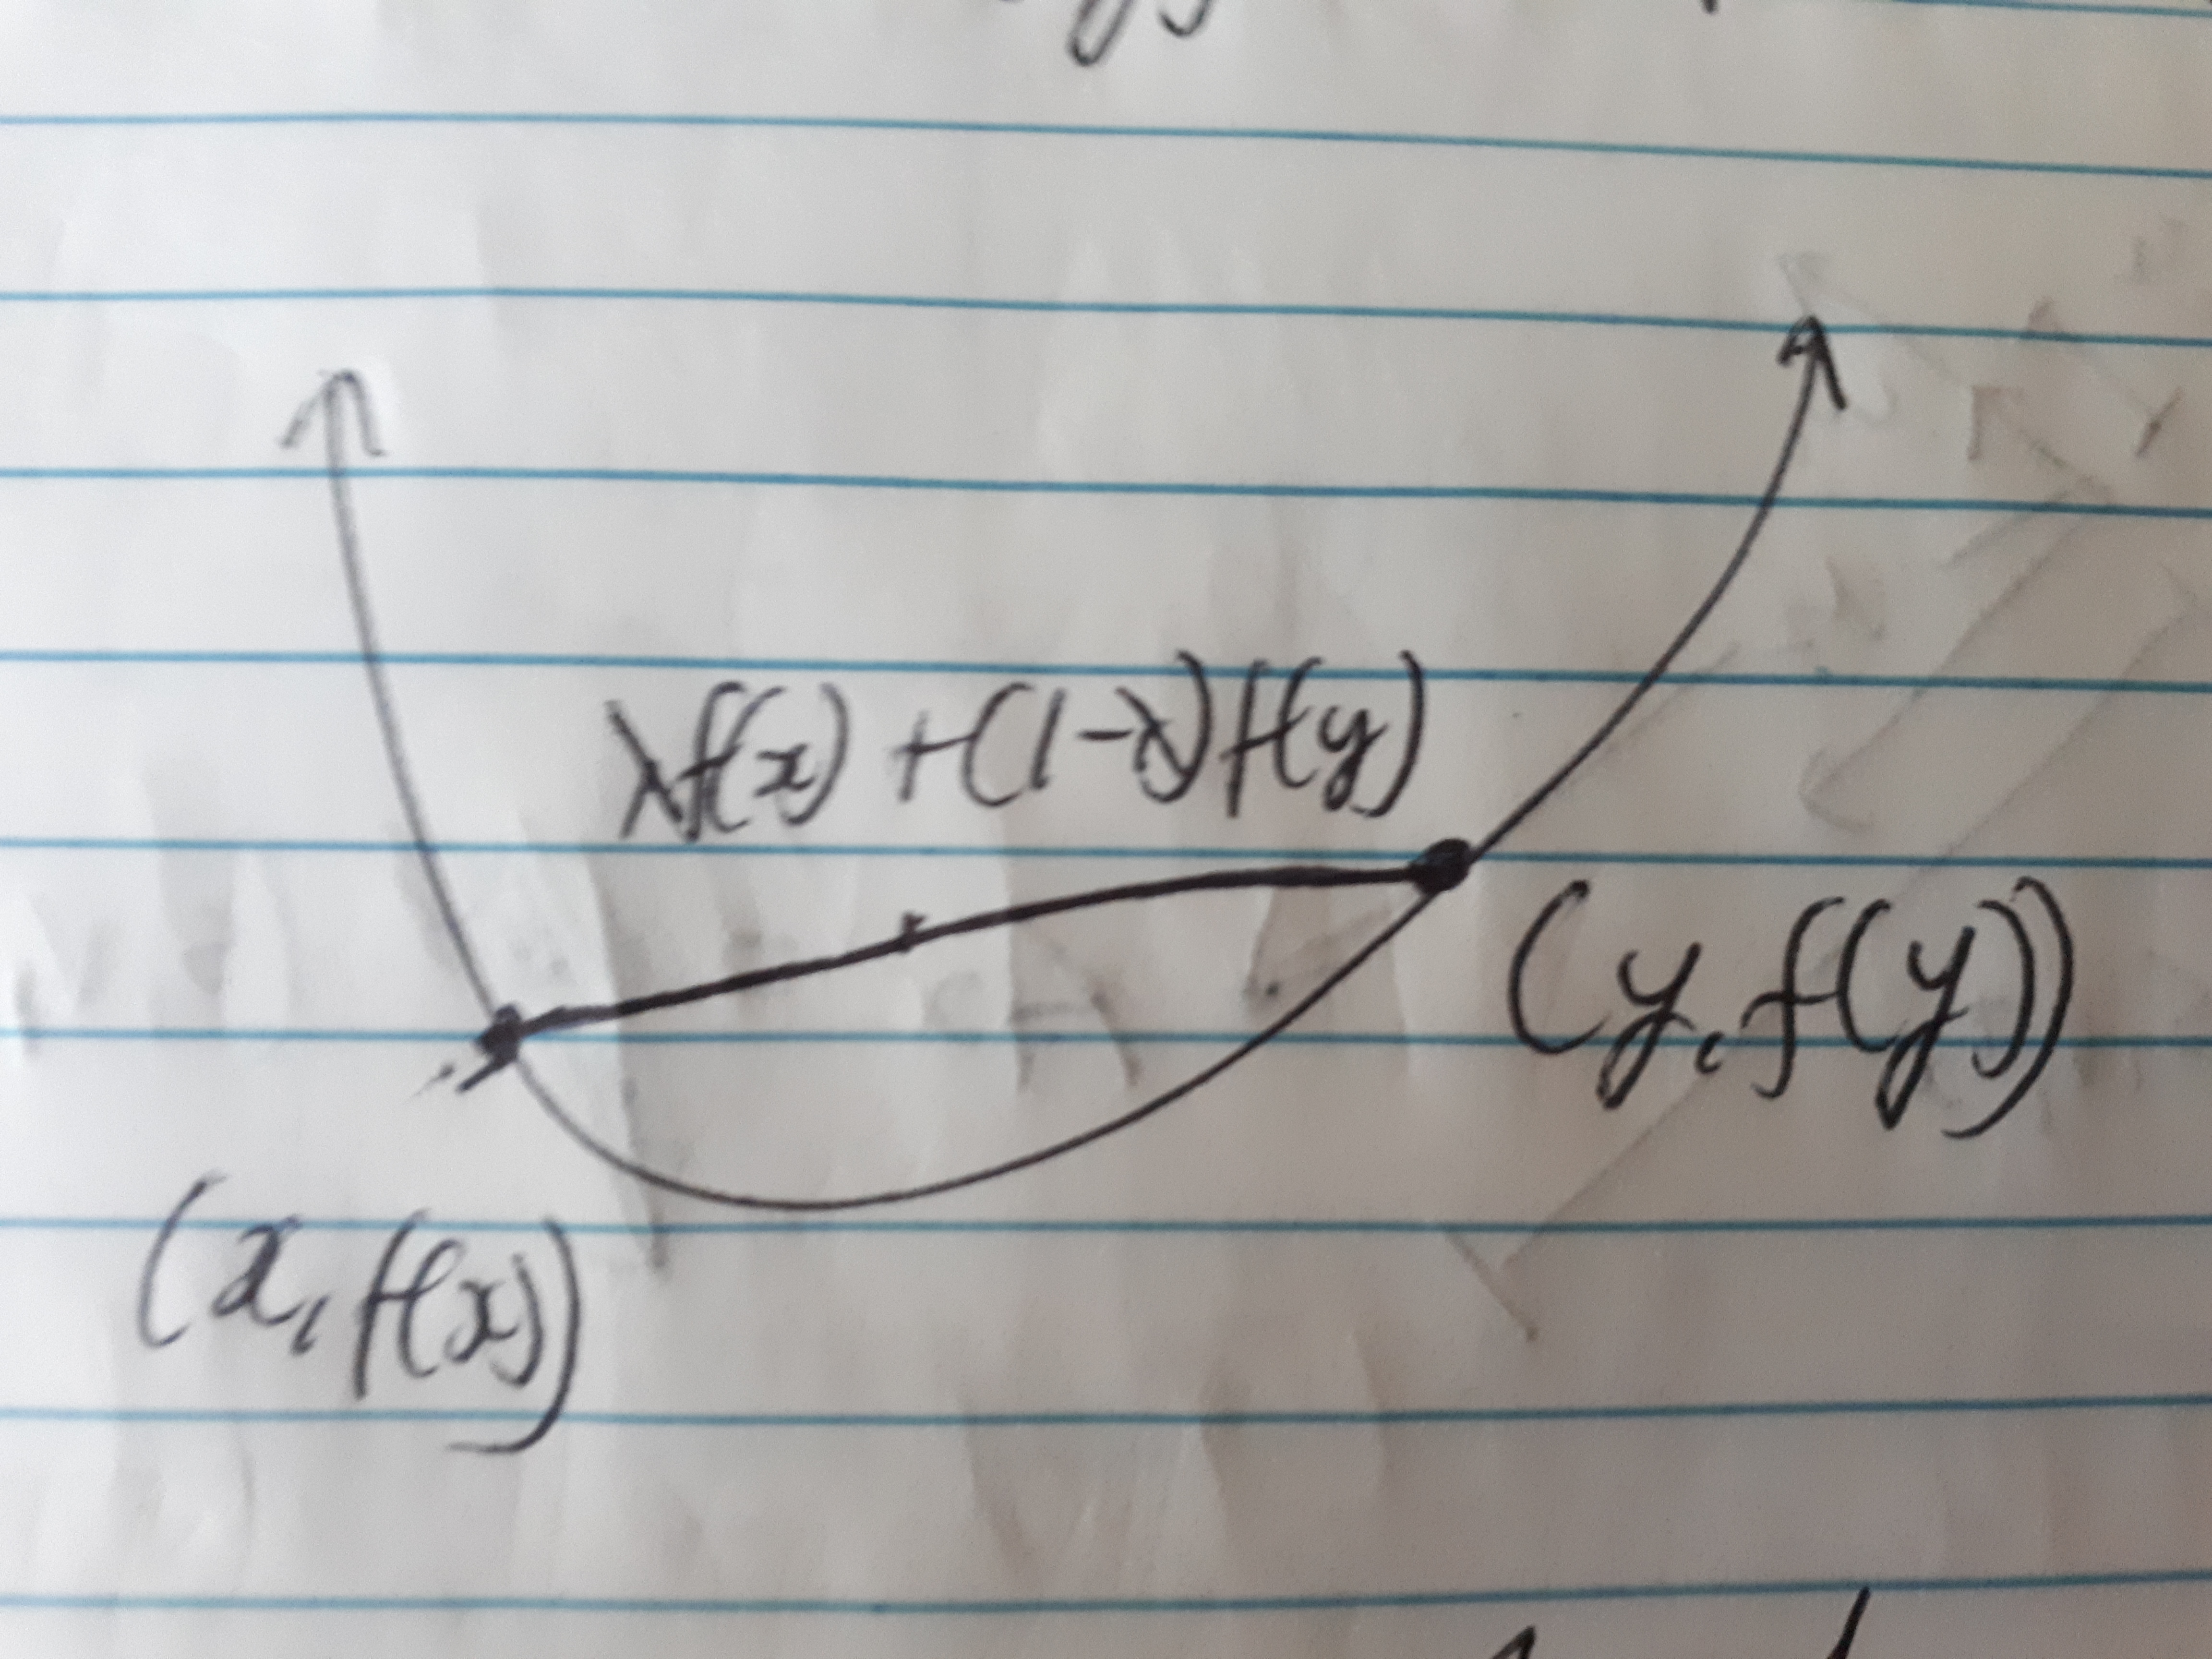
\includegraphics[width = \textwidth/2]{09_28_P02.jpg}
\end{center}
To solve a convex optimisation problem we ``go downhill''. 

\underline{Fact} If $f$ is differentiable, then $f$ is convex if and only if 
\[f(y)\ge f(x) + \nabla f(x)^T(y-x),\]
for all $x$ and $y$. That is the line tangent to $f$ at $x$ lies below the graph of $f$. See picture

\begin{center}
    \includegraphics[width = \textwidth/2]{09_28_P03.jpg}
\end{center}

\underline{Fact 2} If $f$ is $\mathcal{C}^2$ (has 2 continuous derivatives), then $f$ is convex iff $\nabla^2 f(x) \succeq 0$ for all $x$ where $\nabla^2 f(x) = \left[\frac{\partial^2}{\partial x_i \partial x_j}f(x)\right]_{i,j=1}^n$. Also for an $n \times n$ matrix $A \succeq 0$ means $A$ is positive semi-definite i.e. $x^TAx \ge 0$ for all $x \in \R^n$.

\begin{prop}
If $f$ is convex, then $x^*$ minimizes $f$ if and only if $\nabla f(x^*) = 0$.
\end{prop}
\begin{proof}
    If $\nabla f(x^*) = 0$, then for all $y$,
    \[f(y) \ge f(x^*) + \nabla f(x^*)^T(y-x) = f(x^*). \]
    Thus $f(x^*)$ is the minimum value of $f$. The converse is similar.
\end{proof}
\underline{Fact 3} If $f: \R^m \to \R$ is convex, $A \in \R^{m \times n}$ and $b \in \R^m$, then $h: \R^n \to \R$ given by $h(x) := f(Ax+b)$ is convex and 
\[\nabla h(x) = A^T \nabla f(Ax+b). \]
\subsection{Least squares example}
[An answer to a student's question] Suppose we are given the data $X \in \R^{n \times d}$ and $Y \in \R^n$. We have the variable $\beta \in \R^d$ and we wish to minimize
\[L(\beta) = \frac{1}{2}\norm{X\beta-Y}_2^2. \]
The function $L$ is convex in $\beta$ and $\nabla L(\beta) = X^T(X\beta - Y)$. Setting this equal to zero gives $X^TX\beta = X^TY$. These equations are called the normal equations. Thus the minimises of $L$ are the solutions to the normal equations.

If $X$ has rank $d$, then $X^TX$ is invertible and 
\[\beta = (X^TX)^{-1}X^TY, \]
is the unique minimizer of $L$.
\subsection{Geometry of convex functions in higher dimensions}
Let's revisit $f(y) \ge f(x)+\nabla f(x)^T(y-x)$ where $f:\R^2 \to \R$ and so we can graph the points $(y_1,y_2,f(y_1,y_2))$ in $\R^3$. The function $f$ being convex means that this graph looks like a bowl. The set of all points 
\[\left(y_1,y_1, f(x_1,x_2)+\nabla f(x_1,x_2)^T\begin{bmatrix}
    y_1-x_1\\y_2-x_2
\end{bmatrix}\right), \]
is the plane that is tangential to the graph of $f$ at the point $(x_1,x_2,f(x_1,x_2))$. Since $f$ is convex and looks like a bowl, we can think of putting a piece of paper that just touches a point on the underside of the bowl. By convexity this piece of paper never goes inside the bowl and thus
\[f(y) = f(y_1,y_2) \ge (x_1,x_2)+\nabla f(x_1,x_2)^T\begin{bmatrix}
    y_1-x_1\\y_2-x_2
\end{bmatrix} = f(x)+\nabla f(x)^T(y-x). \]
See also this picture
\begin{center}
    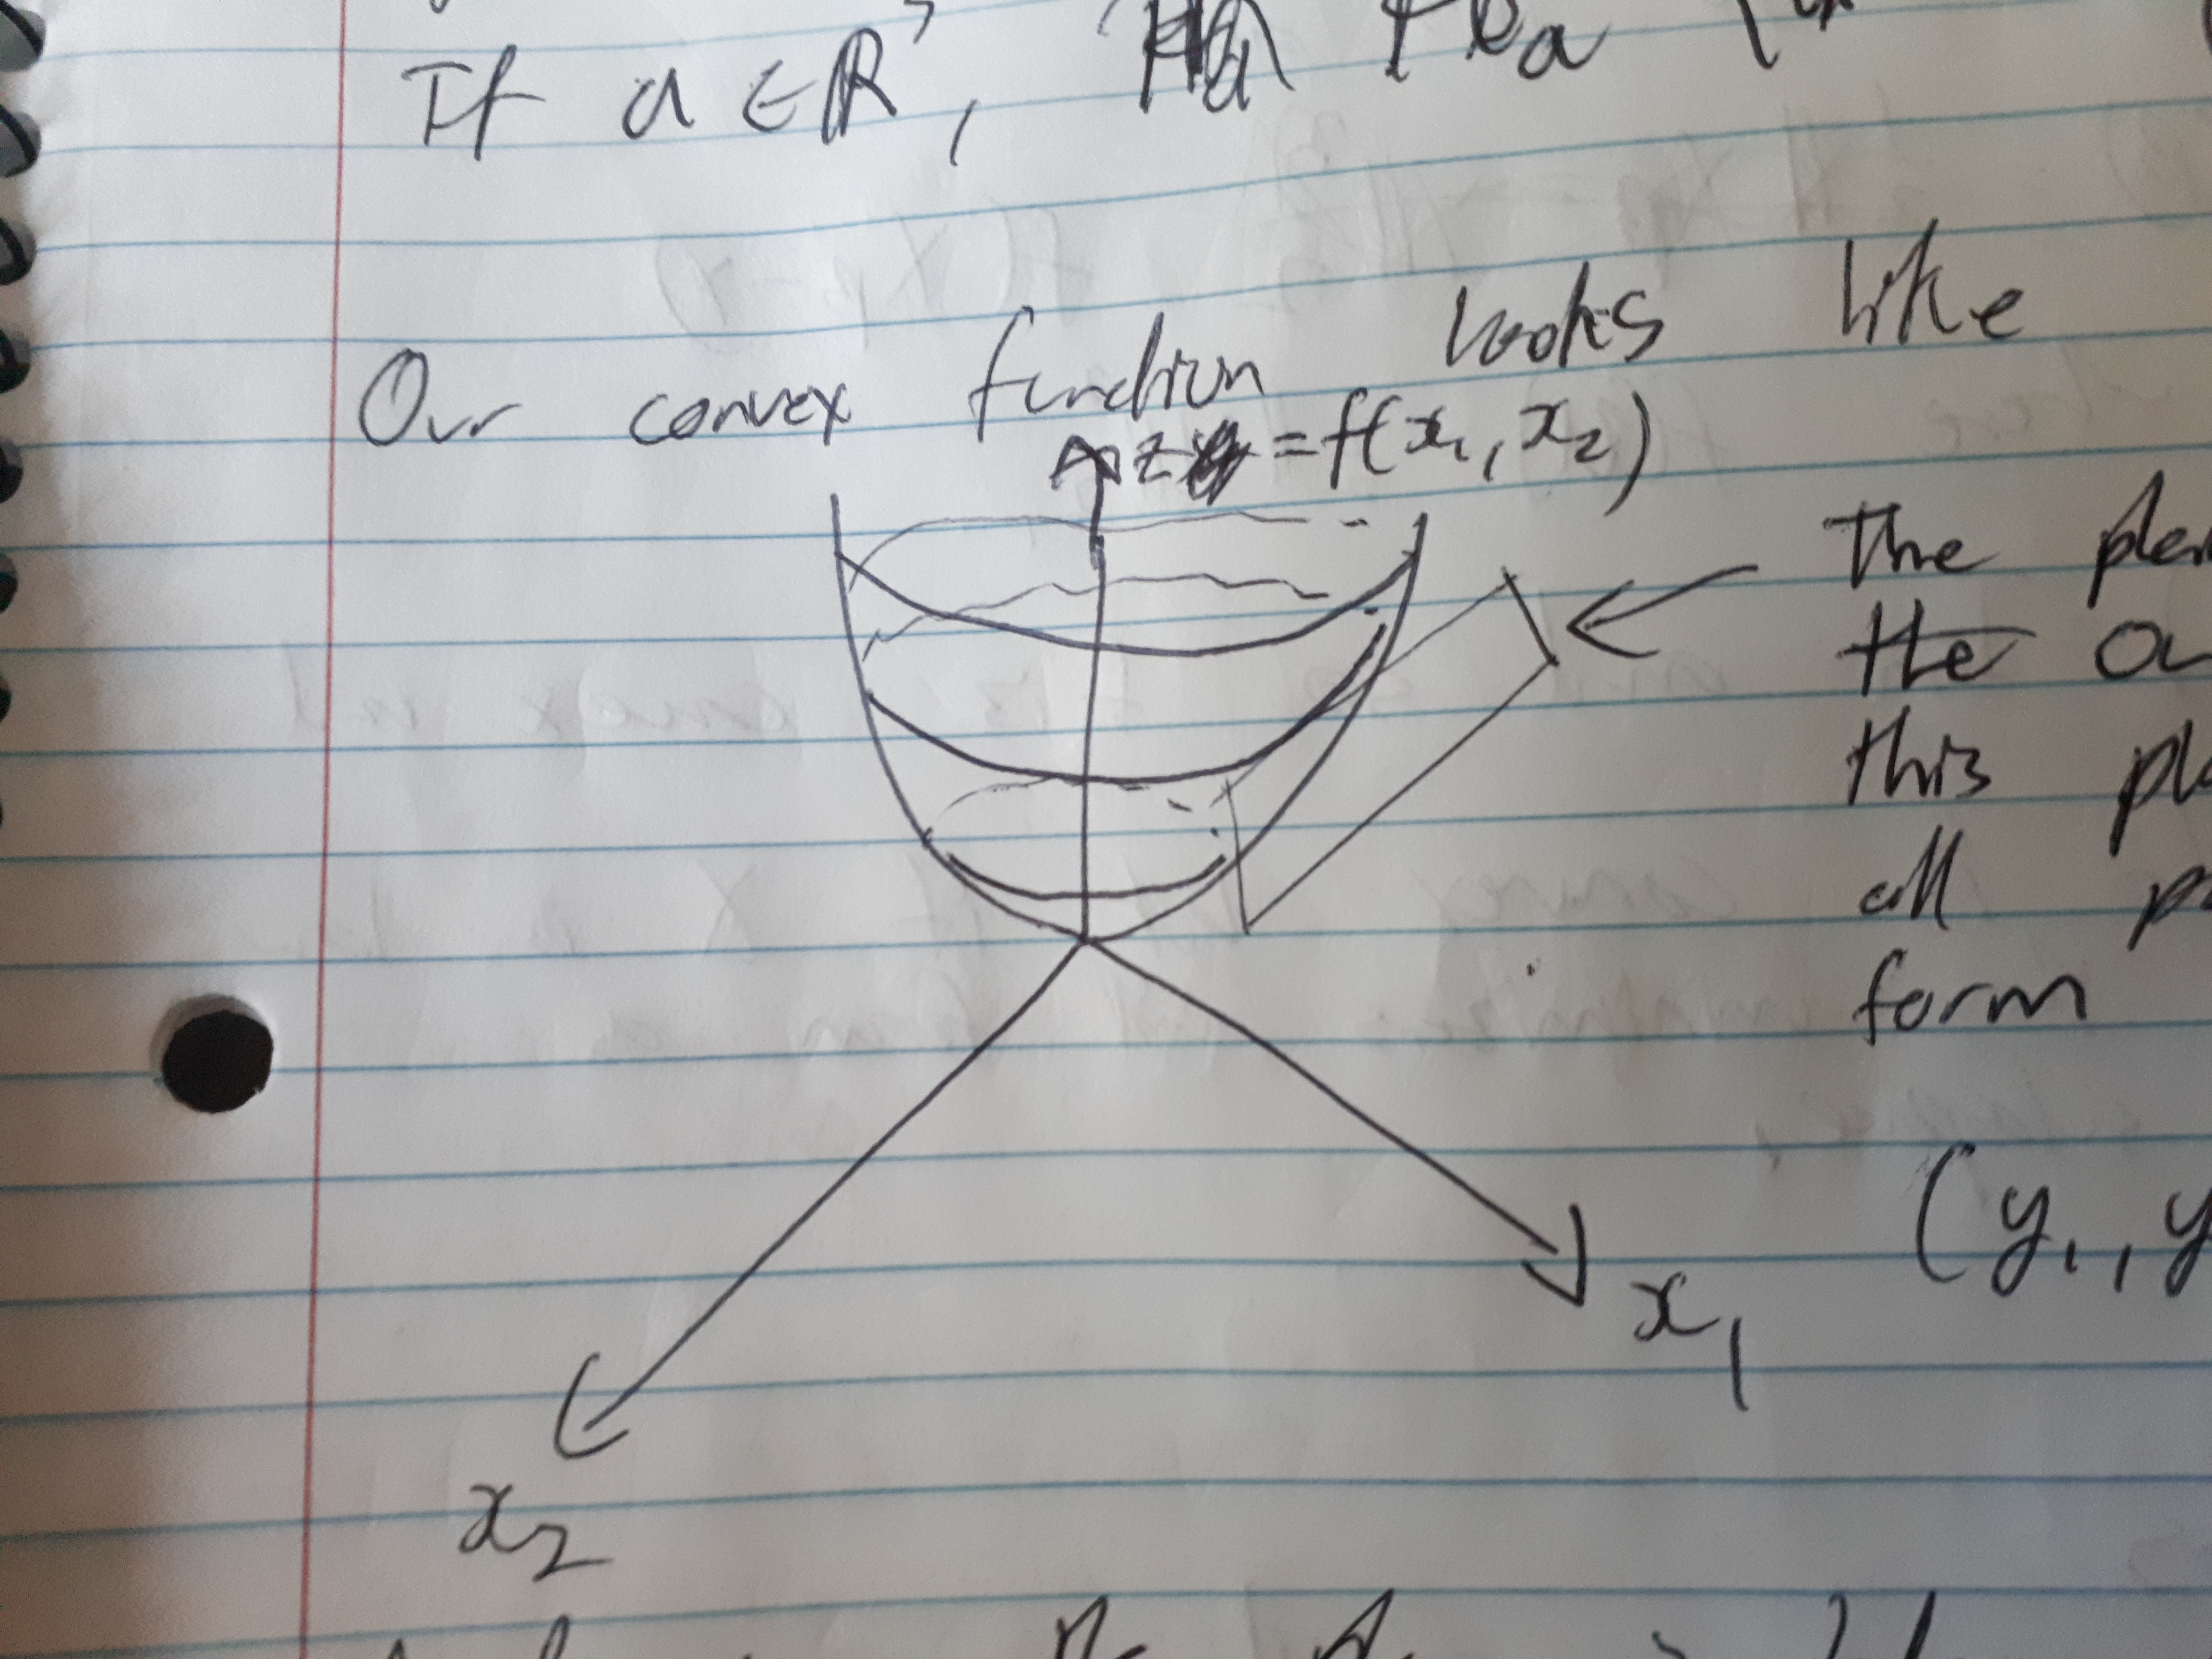
\includegraphics[width = \textwidth/2]{09_28_P04.jpg}
\end{center}
These geometric pictures are useful and important but not something we will be tested on. Note that convex functions may have more than one minimum. 

\subsection{More than one minimum}
See handout on the course webpage for details. In our least squares example we could write 
\[L(\beta) = \frac{1}{2}\norm{X \beta - Y}_2^2, \]
as $L(\beta) = f(X\beta - Y)$ where $f(u) = \frac{1}{2}\norm{u}_2^2$. Since $\nabla^2 f(u) = I_n$, $f$ is convex and thus $L$ is also convex. But if $X$ is rank $r < d$, then there will be multiple solutions to the normal equations and hence multiple minimizers of $L$. These solutions will form an affine subspace. In general the minimizers of a convex function form a convex set.

\subsection{Projections}
Lets consider another problem when we can use the tools of convex optimisation. Given $a_1,\ldots, a_k \in \R^d$ we wish to find the closest point to $v$ in $\spn\{a_i\}_{i=1}^k$. Write $A = [a_1,\ldots, a_n]$, then $x \in \spn\{a_i\}_{i=1}^n$ if and only if $x = A\la$ for some $\la \in \R^k$. Thus our problem is equivalent to the constrained optimisation 
\[\min_{x, \la} \frac{1}{2}\norm{v-x}_2^2 \text{ s.t. } x = A\la. \]
But we can rewrite this as an unconstrained optimisation problem 
\[\min_{\la} \frac{1}{2}\norm{v-A\la}_2^2. \]
We can calculate $\nabla_\la \frac{1}{2}\norm{v-A\la}_2^2 = A^T(A\la - v)$. If $A$ is full rank, then setting $\nabla_\la$ equal to 0 we get $\la = (A^TA)^{-1}A^Tv$ and thus $x = A(A^TA)^{-1}A^Tv$. We can also solve this problem by using the SVD of $A$.

If $A=U\Sigma V^T$ is the SVD of $A$, then
\begin{IEEEeqnarray*}{rCl}
    \Pi_A &:=&A(A^TA)^{-1}A^T\\
    &=&U\Sigma V^T(V\Sigma U^TU\Sigma V^T)^{-1}V\Sigma U^T\\
    &=&U\Sigma V^T(V\Sigma^2V^T)^{-2}V\Sigma U^T\\
    &=&U\Sigma V^TV\Sigma^{-2}V^TV\Sigma U^T\\
    &=&UU^T.
\end{IEEEeqnarray*}
We can also see this because $\spn(A)=\spn(U)$ and projection onto $\spn\{u_1,\ldots, u_k\}$ is 
\[\sum_{i=1}^k u_i(u_i^Tx) = UU^Tx. \]
\subsection{Summary}
This is all the optimisation we will need in this class. It is okay if it was unfamiliar. The upshot is that if we can frame a problem as a convex optimisation problem, then the computer can solve it.
\section{Review of distributions}
A random variable/vector $X \in \R^d$ with a density $f$ or a probability mass function (p.m.f) $p$ has expectation/mean
\[\E[X] = \begin{cases}
    \sum xp(x) & \text{if $X$ has a p.m.f $p$,}\\
    \int xf(x)dx & \text{if $X$ has a density $f$}. 
\end{cases} \]
The random variable $X$ aso has a covariance matrix 
\[\text{Cov}(X) = V(X) = \E[(X-\E X)(X-\E X)^T] = [\text{cov}(X_i,X_j)]_{i,j=1}^d, \]
where $\text{cov}(X_i,X_j) = \E[(X_i-\E X_i)(X_j-\E X_j)]$. Note that $V(X) \succeq 0$ since 
\[u^TV(X)u = \E\left[(u^T(X-\E X))^2\right] \ge 0. \]
\subsection{Normal Distributions}
$X \sim \Na(\mu,\Sigma)$ means that $X$ is normally distributed with expectation $\mu$ and covariance $\Sigma$. This mean $X$ has density
\[f(x) = \frac{1}{(2\pi)^{d/2}\sqrt{\det(\Sigma)}}\exp\left(-\frac{1}{2}(x-\mu)^T\Sigma^{-1}(x-\mu)\right),\]
assuming that $\Sigma \succ 0$, that is $\Sigma$ is positive definite.

Some facts about normal distributions. If $X \sim \Na(0,I)$ and $Y=Ax+b$ then $Y \sim \Na(b, AA^T)$. A ``proof'' $\E[Y] = b$ and 
\[\text{Cov}(Y) = \E[(AX)(AX)^T] = A\E[XX^T]A^T = AA^T.\]
A consequence of this is that normals are rotationally invariant. That is if $U \in \R^{d\times d}$ is orthogonal ($UU^T = I_d$) and $Z \sim \Na(0,I)$, then $UZ \sim \Na(0,I)$. That is $UZ$ and $Z$ have the same distriution.

What does a normal distribution look like?

If $\Sigma = V \Lambda V^T$ and $\Lambda = \diag(\la_1,\ldots, \la_d)$, $\la_1 \ge \la_2 \ge \ldots \ge \la_d > 0$, then the density of $X \sim \Na(0,\Sigma)$ is proportional to $\exp\left(-\frac{1}{2} x^T \Sigma^{-1} x\right)$. We know that $\Sigma^{-1} = V\Lambda^{-1} V^T$. Thus the level sets of $f(x)$ are 
\[\{x : x^T \Sigma^{-1} x = \text{ constant} \} = \{x : (Vx)^T\Lambda^{-1} (Vx) = \text{ constant} \}.   \]
These sets are elipses with axis in the direction $v_1,\ldots, v_d$ and length $\sqrt{\la_1}, \ldots, \sqrt{\la_d}$.
\end{document}